\documentclass[aspectratio=43]{beamer}
\usepackage[english]{babel}
\usepackage{amsthm}
\usepackage{mathtools}
\usepackage{physics}
\usepackage{calligra}
\usepackage{csquotes}
\usepackage{tensor}
\usepackage[thicklines]{cancel}
\usepackage{tcolorbox}
\usepackage{pstricks}
\usepackage{setspace}
\usepackage[backend=biber, bibstyle=nature, sorting=nty, citestyle=numeric-comp]{biblatex} %Custom bibliography
    \addbibresource{bib.bib} %Load references


\DeclareMathAlphabet{\mathcalligra}{T1}{calligra}{m}{n}
\DeclareFontShape{T1}{calligra}{m}{n}{<->s*[2.2]callig15}{}
\newcommand{\scriptr}{\mathcalligra{r}\,}
\newcommand{\boldscriptr}{\pmb{\mathcalligra{r}}\,}
\def\rc{\scriptr}
\def\brc{\boldscriptr}
\def\hrc{\hat\brc}
\newcommand{\ie}{\emph{i.e.}} %id est
\newcommand{\eg}{\emph{e.g.}} %exempli gratia
\newcommand{\rtd}[1]{\ensuremath{\left\lfloor #1 \right\rfloor}}
\newcommand{\dirac}[1]{\ensuremath{\delta \left( #1 \right)}}
\newcommand{\diract}[1]{\ensuremath{\delta^3 \left( #1 \right)}}
\newcommand{\e}{\ensuremath{\epsilon_0}}
\newcommand{\m}{\ensuremath{\mu_0}}
\newcommand{\V}{\ensuremath{\mathcal{V}}}
\newcommand{\prnt}[1]{\ensuremath{\left(#1\right)}} %parentheses
\newcommand{\colch}[1]{\ensuremath{\left[#1\right]}} %square brackets
\newcommand{\chave}[1]{\ensuremath{\left\{#1\right\}}}  %curly brackets

\useoutertheme{infolines}
\useinnertheme{rectangles}
\usefonttheme{professionalfonts}


\definecolor{orange}{HTML}{f28165}
\definecolor{gray}{HTML}{303030}
\definecolor{yellow}{HTML}{f0be52}
\definecolor{lightorange}{HTML}{f19e58}

\renewcommand{\CancelColor}{\color{orange}}

\makeatletter
\newcommand{\mybox}[1]{%
  \setbox0=\hbox{#1}%
  \setlength{\@tempdima}{\dimexpr\wd0+13pt}%
  \begin{tcolorbox}[colback=orange,colframe=orange,boxrule=0.5pt,arc=4pt,
      left=6pt,right=6pt,top=6pt,bottom=6pt,boxsep=0pt,width=\@tempdima]
    \textcolor{white}{#1}
  \end{tcolorbox}
}
\makeatother

\usecolortheme[named=orange]{structure}
\usecolortheme{sidebartab}
\usecolortheme{orchid}
\usecolortheme{whale}
\setbeamercolor{alerted text}{fg=yellow}
\setbeamercolor{block title alerted}{bg=alerted text.fg!90!black}
\setbeamercolor{block title example}{bg=lightorange!60!black}
\setbeamercolor{background canvas}{bg=gray}
\setbeamercolor{normal text}{bg=gray,fg=white}

\setbeamertemplate{footline}
        {
      \leavevmode%
      \hbox{%
      \begin{beamercolorbox}[wd=.25\paperwidth,ht=2.25ex,dp=1ex,center]{author in head/foot}%
        \usebeamerfont{author in head/foot}\insertshortauthor~~(\insertshortinstitute)
      \end{beamercolorbox}%
      \begin{beamercolorbox}[wd=.25\paperwidth,ht=2.25ex,dp=1ex,center]{title in head/foot}%
        \usebeamerfont{title in head/foot}\insertshorttitle
      \end{beamercolorbox}%
      \begin{beamercolorbox}[wd=.25\paperwidth,ht=2.25ex,dp=1ex,center]{date in head/foot}%
        \usebeamerfont{date in head/foot}\insertshortdate{}%\hspace*{2em}

      \end{beamercolorbox}

      \begin{beamercolorbox}[wd=.25\paperwidth,ht=2.25ex,dp=1ex,center]{date in head/foot}%
        % \usebeamerfont{date in head/foot}\insertshortdate{}%\hspace*{2em}
        %
      %#turning the next line into a comment, erases the frame numbers
        \insertframenumber{} / \inserttotalframenumber
        % \hspace*{2ex}
      \end{beamercolorbox}}%
      \vskip0pt%
    }


\setbeamertemplate{blocks}[rectangle]
\setbeamercovered{dynamic}

\setbeamertemplate{section page}
{
	\begin{centering}
		\begin{beamercolorbox}[sep=27pt,center]{part title}
			\usebeamerfont{section title}\insertsection\par
			\usebeamerfont{subsection title}\insertsubsection\par
		\end{beamercolorbox}
	\end{centering}
}

%\setbeamertemplate{subsection page}
%{
%	\begin{centering}
%		\begin{beamercolorbox}[sep=12pt,center]{part title}
%			\usebeamerfont{subsection title}\insertsubsection\par
%		\end{beamercolorbox}
%	\end{centering}
%}

\newcommand{\hlight}[1]{\colorbox{violet!50}{#1}}
\newcommand{\hlighta}[1]{\colorbox{red!50}{#1}}

\title{Dynamic Seat Assignment with Social Distancing} %->->->->-> Check hyperref title <-<-<-<-<-
\subtitle{}
% \author[LI]{LI $\cdot$ Zikang}
\institute[HKUST]{
    IEDA%
    \\%
    The Hong Kong University of Science and Technology%
} %You can change the Institution if you are from somewhere else
\date{}

% \setbeamertemplate{bibliography item}[text]

\begin{document}
    \frame{\titlepage}
    \begin{frame}{Table of Contents}
        \tableofcontents
    \end{frame}
    % !TeX root = ../main.tex

\section{Literature Review}
    \frame{\sectionpage}
    \begin{frame}{Seat Planning with Social Distancing}
      \begin{itemize}
        \item Applications: 

        \vspace*{0.2cm}
        {\color{red} Airplanes} seat planning (Ghorbani et.al 2020)
        
        {\color{red} Classroom} layout planning (Bortolete et al. 2022)
        
        {\color{red} Trains} seat planning (Haque \& Hamid 2022).
        
        \vspace*{0.2cm}

        \item Group-based seat planning for {\color{green}known groups}:
        
        % People in the same {\color{red}group can sit together}: 
        
        % Social distancing can be enforced in different {\color{red}groups} (Moore et al. 2021).
        \vspace*{0.2cm} 

         {\color{red}Amphitheaters} (Haque \& Hamid 2022) 
         
         {\color{red}Airplanes} (Salari et al. 2022) 
         
         {\color{red}Theaters} (Blom et al. 2022).
        
         \vspace*{0.4cm}
        Our work considers seat planning with stochastic demand.
        % \item[] Sitting together as a group does not pose an increased risk of infection
        
      \end{itemize}
      \end{frame}
      
      \begin{frame}{Dynamic Seat Assignment}
        \begin{itemize}
          \item {\color{red}Dynamic multiple} knapsack problem:
                
          \item[-] Multiple knapsack problem (Pisinger et al. 1999)
          
          \item[-] Dynamic knapsack problem (Kleywegt et al. 1998)

          % \vspace*{0.3cm}
          % Our work considers the {\color{red}dynamic form} and {\color{red}multiple rows}.

          \vspace*{0.3cm}

          % \item Dynamic seat assignment on airplane (Notomista et al. 2016), train (Hamdouch et al. 2011).

          \item Network revenue management: {\color{red} Group-based} (Talluri et al. 2006).

          \vspace*{0.5cm}
          \item Dynamic capacity control: {\color{red} Assign-to-seat} for selling high-speed train
          tickets (Zhu et al. 2023)
        \end{itemize}

        \vspace*{0.4cm}

        \qquad Our work considers the group-based seat assignment.
        % train (Hamdouch et al. 2011),  (Berge et al. 1993).
      \end{frame}
    % !TeX root = ../main.tex

\section{Problem Definition}
    \frame{\sectionpage}

    \begin{frame}{Seat Planning with Social Distancing}
      \begin{itemize}
      \item Group type $\mathcal{M} = \{1, \ldots, M\}$.
      \item Row $\mathcal{N} = \{1, \ldots, N\}$.
      \item The number of seats in row $j$: $S_j, j \in \mathcal{N}$.
      \item $\delta$ seat(s) as the social distancing.
      \item Let $n_i = i + \delta$ denote the new size of group type $i$ for each $i \in \mathcal{M}$.
      \item Let $L_j = S_j + \delta$ denote the length of row $j$ for each $j \in \mathcal{N}$.
      \end{itemize}
      
      \begin{figure}[ht]
        \centering
        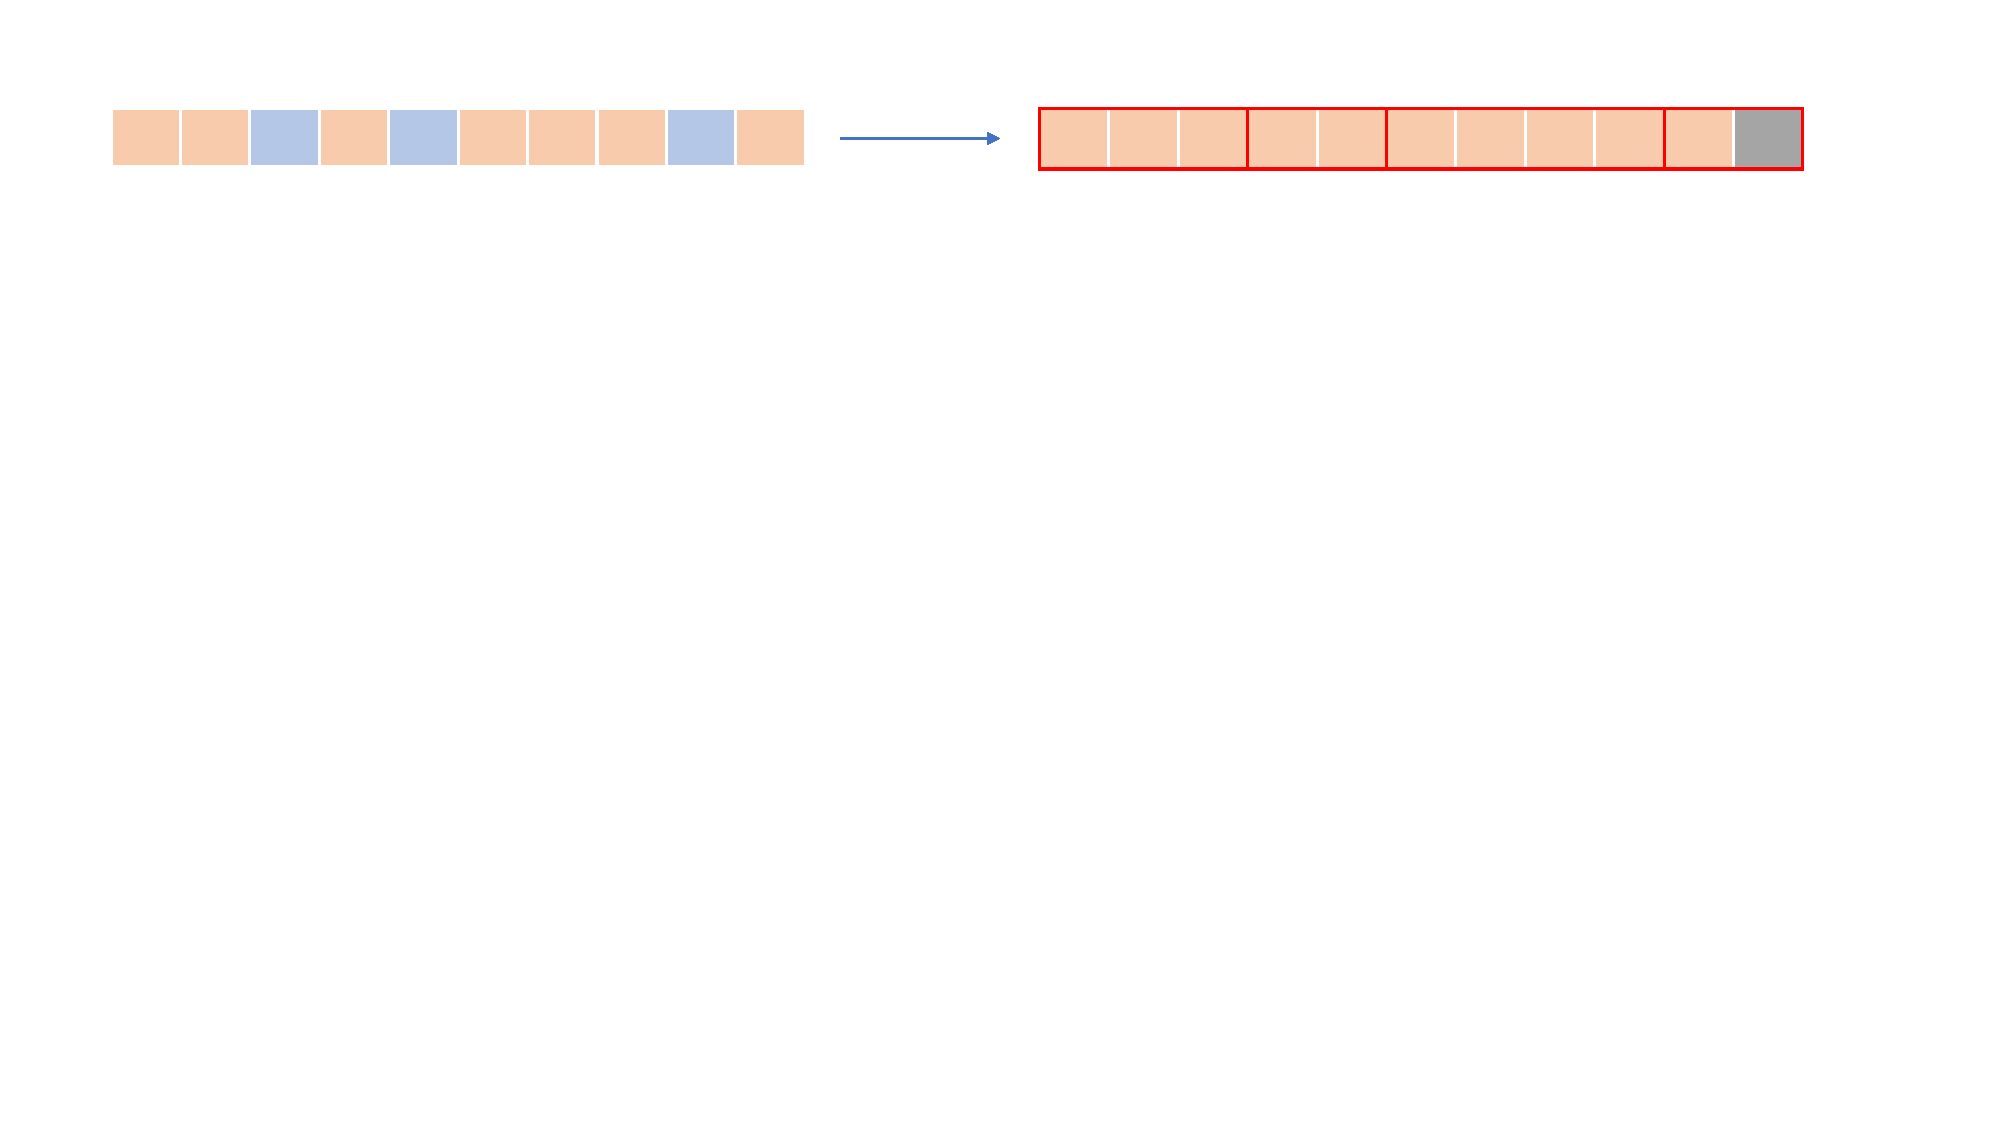
\includegraphics[width = 0.8\textwidth]{./images/dummy_seat.pdf}
        \caption{Problem Conversion with One Seat as Social Distancing}
    \end{figure}
    \end{frame}

  \begin{frame}{Some Definitions}
    \begin{itemize}
      \item Pattern refers to the seat planning for one row.
      \item For each pattern $k$, $\alpha_k, \beta_k$ indicate the number of groups and the left seats, respectively.
      \item Denote by $\alpha_k \delta + \beta_k - \delta$ the loss for pattern k, $l(k)$. The loss represents the number of people lost compared to the situation without social distancing.
      \item Let $I_1$ be the set of patterns with the minimal loss. We call the patterns from $I_1$ are the largest. The patterns with zero left seat are called full patterns.
      \item Suppose there are $n$ groups in a row, for ease of brevity, we use a descending form $P_{k} = (t_1, t_2, \ldots, t_n)$ to denote pattern $k$, where $t_h$ is the new group size, $h = 1,\ldots, n$.
    \end{itemize}
  \end{frame}

  \begin{frame}{Example}
    \begin{itemize}
      \item Suppose the social distancing is one seat and there are four types of groups. Then the new sizes of groups are $2, 3, 4, 5$, respectively. 
      % \item The demand for each group type is $[10, 12, 9, 8]_d$. 
      \item The length of one row is $L = 21$.
      \item Then these patterns, $(5, 5, 5, 5), (5, 4, 4, 4, 4),(5, 5, 5, 3, 3)$, belong to $I_1$.
      \item Pattern $(5, 5, 5, 5)$ is not full because there is one left seat.
    \end{itemize}
  \end{frame}

  \begin{frame}{Loss from Social Distancing}
    \begin{itemize}
      \item The largest pattern can be obtained by the greedy way: select the maximal group size, $n_{M}$, as many times as possible, then $L = n_{M} \cdot q + r, 0 \leq r < n_{M}$, $r$ is the number of empty seats. When $r > \delta$, these seats can be occupied by the group type $(r-\delta)$; when $r \leq \delta$, leave these seats empty.
      \item The loss of the largest pattern is $q \delta -\delta + f(r)$, where $f(r) =0$ if $r > \delta$; $f(r) = r$ if $r \leq \delta$.
      \item For a seat layout, $\{S_1, S_2, \ldots, S_{N}\}$, the minimal total loss is $\sum_{j} (\lfloor \frac{S_j+\delta}{n_{M}} \rfloor -\delta + f((S_j + \delta) \mod n_{M}))$. The maximal number of people assigned is $\sum_{j} (S_j - \lfloor \frac{S_j+\delta}{n_{M}} \rfloor + \delta - f((S_j +\delta)\mod n_{M}))$.
    \end{itemize}
  \end{frame}
  
  \begin{frame}{Dynamic Programming}
    \centering
    Dynamic seat assignment can be characterized by DP:
    $$V_{t}(\mathbf{L}) = \mathbb{E}_{i \sim p}\left[\max_{\substack{j \in \mathcal{N}: \\ L_j \geqslant {n}_{i}}}\left\{V_{t+1}\left(\mathbf{L}- n_{i}\mathbf{e}_j^{\intercal} \right)+ i, V_{t+1}(\mathbf{L})\right\}\right]$$
    $$V_{T+1}(\mathbf{L}) = 0,$$

    \begin{itemize}
      \item $\mathbf{L} = (L^{r}_1, L^{r}_2, \ldots, L^{r}_{N})$, remaining capacity. $L^{r}_{j}$ represents the number of remaining seats in row $j$.
      \vspace{10pt}
      \item $p_i$: the probability of an arrival of group type $i$.
    \end{itemize}
\end{frame}
    % !TeX root = ../main.tex

\section{Seat Planning by Stochastic Programming}
    \frame{\sectionpage}

    \begin{frame}{Method Flow}
      \begin{itemize}
        \item The formulation of scenario-based stochastic programming(SSP).
        \item Reformulate (SSP) to the benders master problem(BMP) and subproblem.
        \item The optimal solution can be obtained by solving (BMP) iteratively.
        \item To avoid solving IP directly, we consider the LP relaxation form. 
        \item Obtain integral seat planning by deterministic model.
      \end{itemize}
    \end{frame}

    \begin{frame}{Scenario-based Stochastic Programming}
      \footnotesize
      \begin{equation}\label{sto_form}
        \begin{aligned}
       (SSP) \max \quad & E_{\omega}\left[\sum_{i=1}^{M-1} (n_i-\delta) (\sum_{j= 1}^{N} x_{ij} + y_{i+1,\omega}^{+} - y_{i \omega}^{+}) + (n_{M}-\delta) (\sum_{j= 1}^{N} x_{Mj} - y_{M \omega}^{+})\right] \\
        \text {s.t.} \quad & \sum_{j= 1}^{N} x_{ij}-y_{i \omega}^{+}+
        y_{i+1, \omega}^{+} + y_{i \omega}^{-}=d_{i \omega}, \quad i = 1,\ldots,M-1, \omega \in \Omega \\
        & \sum_{j= 1}^{N} x_{ij} -y_{i \omega}^{+}+y_{i \omega}^{-}=d_{i \omega}, \quad i = M, \omega \in \Omega \\
        & \sum_{i=1}^{M} n_{i} x_{ij} \leq L_j, j \in \mathcal{N}\\
        & y_{i \omega}^{+}, y_{i \omega}^{-} \in \mathbb{Z}_{+}, \quad i \in \mathcal{M}, \omega \in \Omega \\
        & x_{ij} \in \mathbb{Z}_{+}, \quad i \in \mathcal{M}, j \in \mathcal{N}.
        \end{aligned}
      \end{equation}
    \end{frame}

\begin{frame}{Reformulation}
  \begin{equation}\label{BD_master}
    \begin{aligned}
  \max \quad & \mathbf{c}^{\intercal} \mathbf{x}+ z(\mathbf{x}) \\
  \text {s.t.} \quad & \mathbf{n} \mathbf{x} \leq \mathbf{L} \\
  & \mathbf{x} \in \mathbb{Z}_{+}^{M \times N},
  \end{aligned}
  \end{equation}

  where $z(\mathbf{x})$ is defined as 

$$z(\mathbf{x}) := E(z_{\omega}(\mathbf{x})) = \sum_{\omega \in \Omega} p_{\omega} z_{\omega}(\mathbf{x}),$$ and for each scenario $\omega \in \Omega$, 

  \begin{equation}\label{BD_sub}
    \begin{aligned}
      z_{\omega}(\mathbf{x}) := \max \quad & \mathbf{f}^{\intercal} \mathbf{y} \\
      \text {s.t.} \quad & \mathbf{x} \mathbf{1} + \mathbf{V} \mathbf{y} = \mathbf{d}_{\omega} \\
       & \mathbf{y} \geq 0.
    \end{aligned}
    \end{equation}
\end{frame}

\begin{frame}{Solution to Subproblem}
  Problem (3) is easy to solve with a given $\mathbf{x}$ which can be seen by the dual problem:

  \begin{equation}\label{BD_sub_dual}
    \begin{aligned}
      \min \quad & \alpha^{\intercal}_{\omega} (\mathbf{d}_{\omega}- \mathbf{x} \mathbf{1}) \\
      \text {s.t.} \quad & \alpha^{\intercal}_{\omega} \mathbf{V} \geq \mathbf{f}^{\intercal}
    \end{aligned}
    \end{equation}

    \begin{itemize}
      \item The feasible region of problem \eqref{BD_sub_dual}, $P= \{\alpha|\alpha^{\intercal} V \geq \mathbf{f}^{\intercal}\}$, is bounded. In addition, all the extreme points of $P$ are integral.
      \item The optimal solution to this problem can be obtained directly according to the complementary slackness property.
    \end{itemize}
\end{frame}

\begin{frame}{Bneders Decomposition Procedure}
  \small
  (SSP) can be obtained by solving following restricted benders master problem(BMP):
  \begin{equation}\label{BD_master2}
    \begin{aligned}
      \max \quad & \mathbf{c}^{\intercal} \mathbf{x} + \sum_{\omega \in \Omega} p_{\omega} z_{\omega} \\
      \text {s.t.} \quad & \mathbf{n} \mathbf{x} \leq \mathbf{L} \\
      & (\alpha^{k})^{\intercal}(\mathbf{d}_{\omega}- \mathbf{x} \mathbf{1}) \geq z_{\omega}, \alpha^k \in \mathcal{O}, \forall \omega \\
       & \mathbf{x} \in \mathbb{Z}_{+}
    \end{aligned}
  \end{equation} 

  Constraints will be generated from problem \eqref{BD_sub_dual} until an optimal solution is found.

  \begin{figure}[ht]
    \centering
    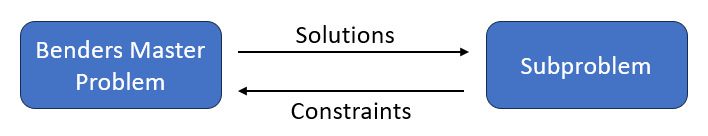
\includegraphics[width = 0.6\textwidth]{./images/BD.png}
  \end{figure}

  To avoid solving IP directly, we consider the LP relaxation of Problem \eqref{BD_master2}.
\end{frame}

% \begin{frame}{Deterministic Formulation}
%   Substitute the first constraint with $\sum_{j= 1}^{N} x_{ij} \geq s_{i}, i \in \mathcal{M}$, we can obtain the problem with lower bound supply. 
% \end{frame}

\begin{frame}{Deterministic Formulation}  %开始一张幻灯片
  To obtain an integral seat planning, we consider the following two deterministic formulations.
  \begin{columns}[c]  %开始进入分栏环境,居中设置
  \column{5cm}  %第一栏(左栏)宽度为5cm
  \scriptsize
  \begin{equation}\label{deter_upper}
    \begin{aligned}
    \max \quad & \sum_{i=1}^{M}  \sum_{j= 1}^{N} (n_i- s) x_{ij} \\
    \text {s.t.} \quad & \sum_{j= 1}^{N} x_{ij} {\color{red} \leq} s_{i}^{0}, \quad i \in \mathcal{M}, \\
    & \sum_{i=1}^{M} n_{i} x_{ij} \leq L_j, j \in \mathcal{N} \\
    & x_{ij} \in \mathbb{Z}_{+}, \quad i \in \mathcal{M}, j \in \mathcal{N}.
    \end{aligned}
  \end{equation}
  \column{5cm}
  \scriptsize
  \begin{equation}\label{deter_lower}
    \begin{aligned}
    \max \quad & \sum_{i=1}^{M}  \sum_{j= 1}^{N} (n_i- s) x_{ij} \\
    \text {s.t.} \quad & \sum_{j= 1}^{N} x_{ij} {\color{red} \geq} s_{i}^{1}, \quad i \in \mathcal{M}, \\
    & \sum_{i=1}^{M} n_{i} x_{ij} \leq L_j, j \in \mathcal{N} \\
    & x_{ij} \in \mathbb{Z}_{+}, \quad i \in \mathcal{M}, j \in \mathcal{N}.
    \end{aligned}
  \end{equation}
  \end{columns}  %分栏环境结束
  Problem \eqref{deter_upper} can generate a feasible seat planning.

  Problem \eqref{deter_lower} can generate a seat planning no inferior than any given feasible seat planning.
\end{frame}


\begin{frame}{Obtain The Feasible Seat Planning}
      \begin{description}
        \item[Step 1.] Obtain the solution, $\mathbf{x}^{*}$, by benders decomposition. Aggregate $\mathbf{x}^{*}$ to the number of each group type, ${s}_{i}^{0} =\sum_{j} x^{*}_{ij}, i \in \mathbf{M}$.

        \item[Step 2.] Solve problem \eqref{deter_upper} to obtain the optimal solution, $\mathbf{x}^{1}$. Aggregate $\mathbf{x}^{1}$ to the number of each group type, ${s}_{i}^{1} = \sum_{j} x^{1}_{ij}, i \in \mathbf{M}$.
        
        \item[Step 3.] Solve problem \eqref{deter_lower} to obtain the optimal solution, $\mathbf{x}^{2}$. Aggregate $\mathbf{x}^{2}$ to the number of each group type, ${s}_{i}^{2} = \sum_{j} x^{2}_{ij}, i \in \mathbf{M}$.
    
        \item[Step 4.] For each row, construct a full pattern.
     \end{description}
\end{frame}
    % !TeX root = ./main.tex

\section{Dynamic Seat Assignment for Each Group Arrival}
    \frame{\sectionpage}

    \begin{frame}{Group-type(Supply) Control}
    Feasible seat planning represents the supply for each group type. We can use supply control to
determine whether to accept a group. Specifically, if there is a supply available for an arriving group, we will accept the group. However, if there is no corresponding supply for the arriving group, we need to decide whether to use a larger group supply to meet the group’s needs. When a group is accepted to occupy larger-size seats, the remaining empty seat(s) can be reserved for future demand.
    
The difference of expected number of accepted people between acceptance and rejection on group $i$ occupying $(j+\delta)$-size seats: $d(i,j) = i + (j-i-\delta)P(D_{j-i-\delta} \geq x_{j-i-\delta}+1) - j P(D_{j} \geq x_{j})$ if $j \geq i+\delta$; otherwise, $d(i,j) = i - j P(D_{j} \geq x_{j})$.
Find $d(i,j^{*}) = \max_{j} d(i,j)$, if $d(i,j^{*}) > 0$, accept group type $i$ in $(j^{*}+\delta)$-size seats; otherwise, reject it.
      \end{frame}

\begin{frame}{Stochastic Planning Policy}
  Stochastic planning policy involves using the objective value of accepting or rejecting an arrival to make a decision. To determine this objective value, we need to consider the potential outcomes that could result from accepting the current arrival (i.e., the Value of Acceptance), as well as the potential outcomes that could result from rejecting it (i.e., the Value of Rejection).

  The Value of Acceptance considers the scenarios that could arise if we accept the current arrival, while the Value of Rejection considers the same scenarios if we reject it. By comparing the Value of Acceptance and the Value of Rejection, we can make an informed decision about whether to accept or reject the arrival based on which option has the higher objective value.
\end{frame}

    \begin{frame}{Dynamic Seat Assignment for Each Group Arrival}
        \begin{description}
          \item[Step 1.] Obtain the set of patterns, $\mathbf{P} = \{P_1,\ldots,P_{N}\}$, from the feasible seat planning algorithm. The corresponding aggregate supply is $\mathbf{X} = [x_{1}, \ldots, x_{M}]$.
          \item[Step 2.] For the arrival group type $i$ at period $T{'}$, 
          If $\exists k \in \mathcal{N}$ such that $i \in P_k$, accept the group, update $P_{k} = P_{k}/(i)$ and $x_{i} = x_{i} -1$. Go to step 4. Otherwise, go to step 3.
          \item[Step 3.] Calculate $d(i,j^{*})$. If $d(i,j^{*})>0$, find the first $k \in \mathcal{N}$ such that $j^{*} \in P_k$. If value of acceptance is larger than value of rejection, accept group type $i$ and update $P_{k} = P_{k}/(j^{*})$, $x_{j^{*}} = x_{j^{*}} -1$. Then update $x_{j^{*}-i-\delta} = x_{j^{*}-i-\delta} + 1$ and $P_{k}= P_{k} \cup (j^{*}-i-\delta)$ when $j^{*}-i-\delta > 0$. If $d(i,j^{*}) \leq 0$, reject group type $i$.
          \item[Step 4.] If $T{'} \leq T$, move to next period, set $T{'} = T{'}+1$, go to step 2. Otherwise, terminate this algorithm.
        \end{description}
      \end{frame}
      
      \begin{frame}{Bid-price Control}
        The dual problem of linear relaxation of problem \eqref{deter_upper} is:
        \begin{equation}\label{bid-price_dual}
          \begin{aligned}
          \min \quad & \sum_{i=1}^{M} d_i z_i + \sum_{j= 1}^{N} L_j \beta_{j} \\
          \text {s.t.} \quad & z_{i} + \beta_j n_i \geq (n_i-\delta), \quad i \in \mathcal{M}, j \in \mathcal{N} \\
          & z_{i} \geq 0, i \in \mathcal{M}, \beta_{j} \geq 0, j \in \mathcal{N}.
          \end{aligned}
        \end{equation}
        \small There exists $h$ such that the aggregate optimal solution to relaxation of problem \eqref{deter_upper} takes the form $x e_{h} + \sum_{i=h+1} ^{M} d_{i} e_{i}$, $x = (L- \sum_{i = h+1}^{M} {d_i n_i})/ n_h$.

        The bid-price control policy will make the decision to accept group type $i$, where $i$ is greater than or equal to $h$, if the capacity allows.
      \end{frame}

      \begin{frame}{Dynamic Programming Base-heuristic}
        Relax all rows to one row with the same capacity by $L = \sum_{j=1}^{N} L_j$.
        
        Deterministic problem is: $\{\max \sum_{i=1}^{M} (n_i- \delta) x_{i}: x_{i} \leq d_{i}, i \in \mathcal{M}, \sum_{i=1}^{M} n_{i} x_{i} \leq L, x_{i} \in \mathbb{Z}_{+}\}$.
        
        Let $u$ denote the decision, where $u(t) = 1$ if we accept a request in period $t$, $u(t) =0$ otherwise, the DP with one row can be expressed as:
        $$V_{t}(L) = \mathbb{E}_{i \sim p} [\max_{u \in \{0,1\}} \{ {[V_{t+1}(L-n_i u)+ i u]}\}], L \geq 0$$ 
        $$V_{T+1}(x) =0, \forall x.$$

        After accepting one group, assign it in some row arbitrarily when the capacity of the row allows.
      \end{frame}
      
    % !TeX root = ../main.tex

      
    \begin{frame}{Performances of Different Policies}
        \scriptsize
        $M =4$, $\delta =1$, $N =10$, $L_j =21, j \in \mathcal{N}$, $p_0 = 0$, $|\Omega| = 1000$.
        \begin{table}[ht]
          \centering
          \begin{tabular}{|l|l|l|l|l|l|l|}
          \hline
           T & Probabilities & DSA (\%) & DP1 (\%) & Bid (\%) & Booking (\%) & FCFS (\%) \\
          \hline
          60  & [0.25, 0.25, 0.25, 0.25]  & 99.12 & 98.42 & 98.38 & 96.74 & 98.17 \\
          70  &   & 98.34 & 96.87 & 96.24 & 97.18 & 94.75 \\
          80  &   & 98.61 & 95.69 & 96.02 & 98.00 & 93.18 \\
          90  &   & 99.10 & 96.05 & 96.41 & 98.31 & 92.48 \\
          100 &   & 99.58 & 95.09 & 96.88 & 98.70 & 92.54 \\
          \hline
          60  & [0.25, 0.35, 0.05, 0.35]  & 98.94 & 98.26 & 98.25 & 96.74 & 98.62 \\
          70  &   & 98.05 & 96.62 & 96.06 & 96.90 & 93.96 \\
          80  &   & 98.37 & 96.01 & 95.89 & 97.75 & 92.88 \\
          90  &   & 99.01 & 96.77 & 96.62 & 98.42 & 92.46 \\
          100 &   & 99.23 & 97.04 & 97.14 & 98.67 & 92.00 \\
          \hline
          60  & [0.15, 0.25, 0.55, 0.05]  & 99.14 & 98.72 & 98.74 & 96.61 & 98.07 \\
          70  &   & 99.30 & 96.38 & 96.90 & 97.88 & 96.25 \\
          80  &   & 99.59 & 97.75 & 97.87 & 98.55 & 95.81 \\
          90  &   & 99.53 & 98.45 & 98.69 & 98.81 & 95.50 \\
          100 &   & 99.47 & 98.62 & 98.94 & 98.90 & 95.25 \\
          \hline
          \end{tabular}
        \end{table}
        DSA has better performance than other policies under different demands.

    \end{frame}
      
    \begin{frame}{Impact of Social Distancing as Demand Increases}
        \scriptsize
        $\gamma = p_1 * 1 + p_2 * 2 + p_3 * 3 + p_4 * 4$: the expected number of people at each period.
        \begin{figure}[h]
            \centering
            \subfigure[When $\gamma =2.5$]{
              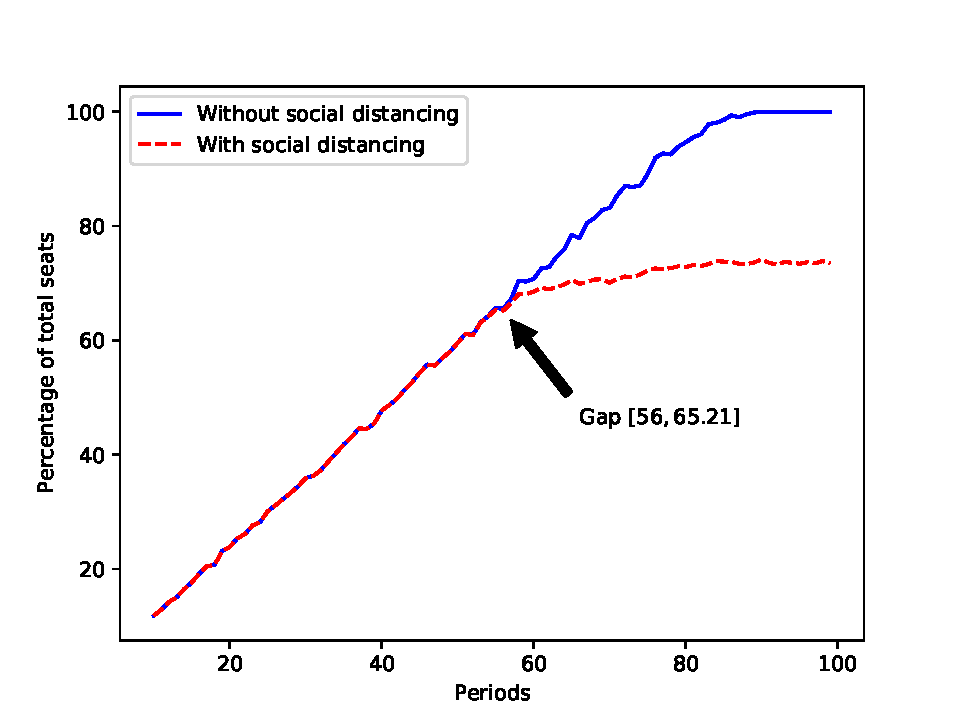
\includegraphics[width=0.48\textwidth]{./images/p1.pdf}}
            \subfigure[When $\gamma =1.9$]{
              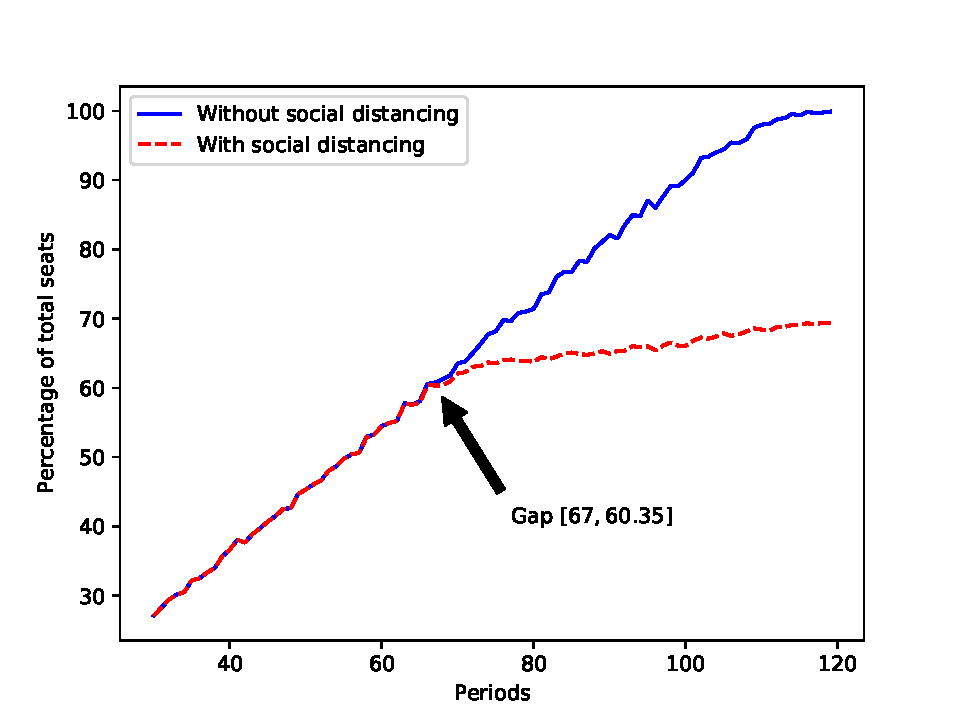
\includegraphics[width=0.48\textwidth]{./images/p2.pdf}}
          \end{figure}
        \scriptsize
        The gap point represents the first period where the number of people without social distancing is larger than that with social distancing and the gap percentage is the corresponding percentage of total seats.
    \end{frame}
      
    \begin{frame}{Estimation of Gap Point}
      \begin{figure}[ht]
        \centering
        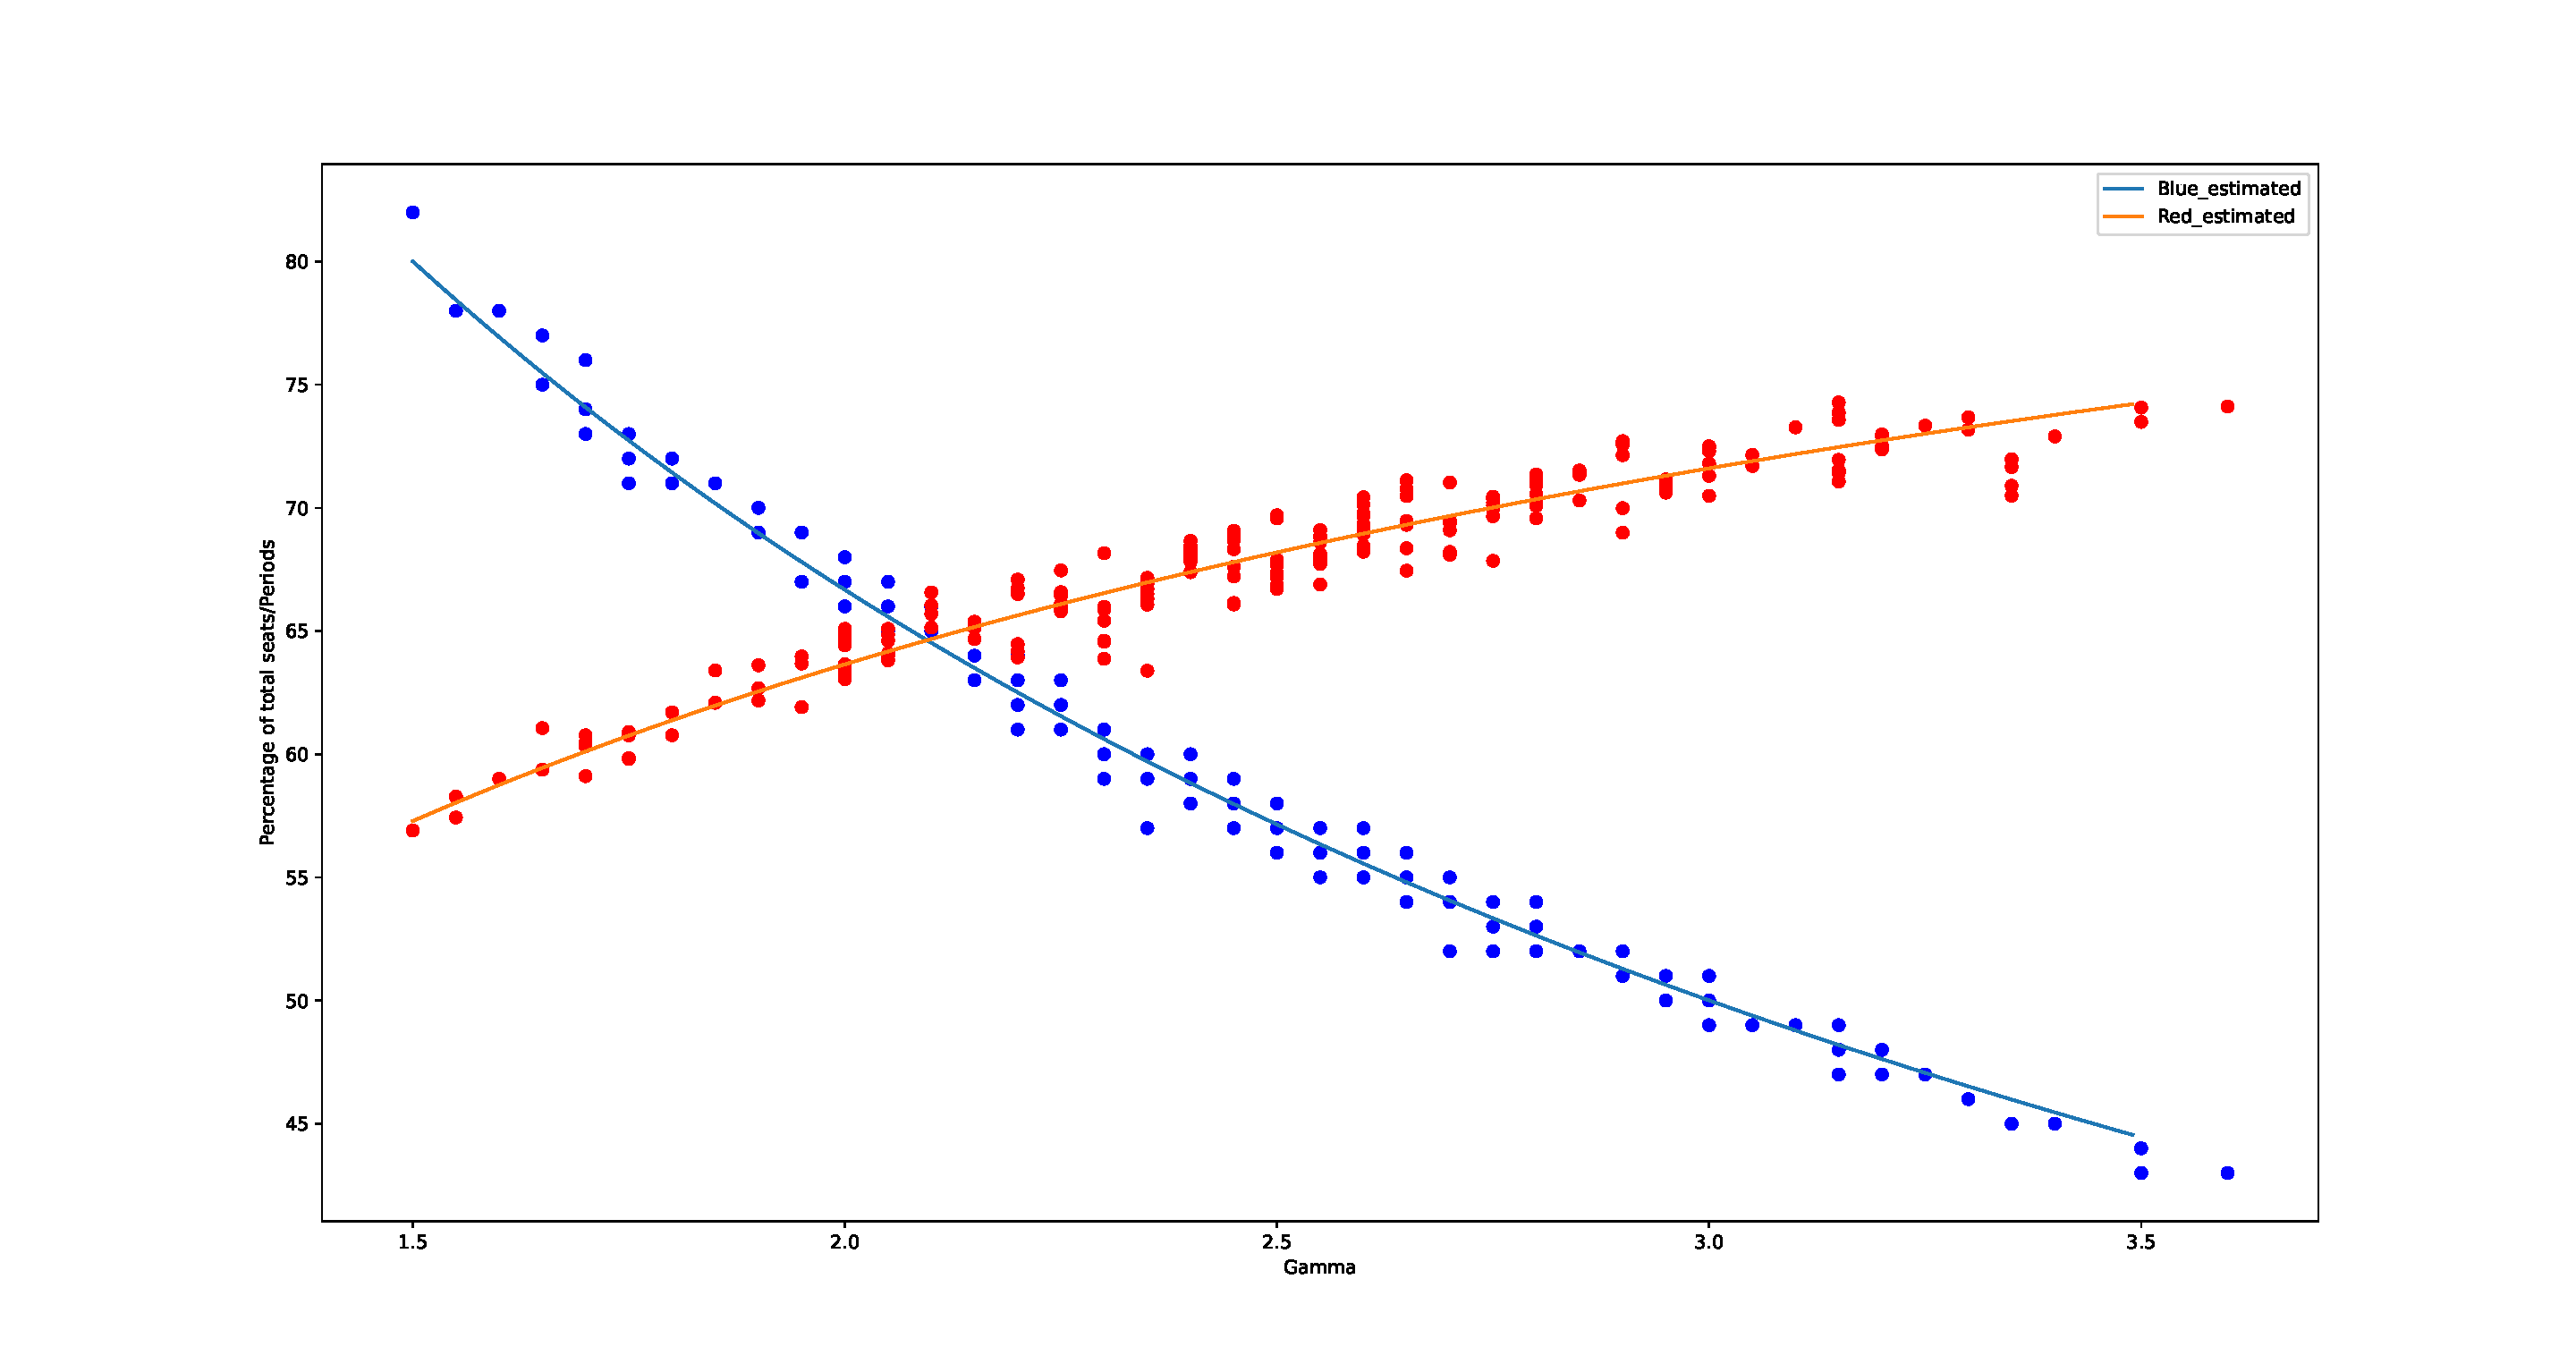
\includegraphics[width = 0.8\textwidth]{./images/gamma_estimation.pdf}
        \caption{Gap points with 200 probabilities}
    \end{figure}
    \scriptsize
    {\color{blue} Blue points}: period of the gap point.
    {\color{red} Red points}: occupancy rate of the gap point. 
    Gap points can be estimated.
    \end{frame}

    % We simulate 200 probabilities. For each probability, we run 100 instances to calculate the gap point and the corresponding occupancy rate. 
    
    % The point in the figure is the average of 100 instances. 
    % 


    \begin{frame}{Make A Later Allocation}
      This setting is particularly applicable to larger venues, such as stadiums, where an immediate decision is made when a group arrives, but the actual allocation of seats for that group is deferred to a later time.

      \vspace{0.5cm}

      The critical part is to make the decision, thus, we choose the following policies associated with relaxation forms.

      \vspace{0.5cm}

      Policies: 

      \begin{itemize}
        \item Dynamic programming based heuristic
        \item Bid-price control
      \end{itemize}
    \end{frame}

      \begin{frame}{Performances of Different Policies}
        \scriptsize
        \begin{table}[ht]
          \centering
          \begin{tabular}{|l|l|l|l|l|l|}
          \hline
           T & Probabilities &  DP1-L (\%) & Bid-L (\%) & DP1 (\%) & Bid (\%) \\
          \hline
          60  & [0.25, 0.25, 0.25, 0.25]  & 99.52 & 99.44 & 98.42 & 98.38 \\
          70  &   & 99.32 & 98.97 & 96.87 & 96.24 \\
          80  &   & 99.34 & 99.30 & 95.69 & 96.02 \\
          90  &   & 99.55 & 99.49 & 96.05 & 96.41  \\
          100 &   & 99.78 & 99.66 & 95.09 & 96.88 \\
          \hline
          60  & [0.25, 0.35, 0.05, 0.35]  & 99.50 & 99.37 & 98.26 & 98.25  \\
          70  &   & 99.40 & 98.97 & 96.62 & 96.06 \\
          80  &   & 99.46 & 99.24 & 96.01 & 95.89 \\
          90  &   & 99.59 & 99.35 & 96.77 & 96.62 \\
          100 &   & 99.77 & 99.61 & 97.04 & 97.14  \\
          \hline
          60  & [0.15, 0.25, 0.55, 0.05]  & 99.57 & 99.54 & 98.72 & 98.74 \\
          70  &   & 99.46 & 99.39  & 96.38 & 96.90 \\
          80  &   & 99.50 & 99.30  & 97.75 & 97.87 \\
          90  &   & 99.34 & 99.44  & 98.45 & 98.69 \\
          100 &   & 99.34 & 99.55  & 98.62 & 98.94 \\
          \hline
          \end{tabular}
        \end{table}

    \end{frame}
    %You can put the frames directly into the presentation, but using the input command and writing them in separate .tex files might be more organized

    % \begin{frame}{Reference}
    %     \printbibliography
    % \end{frame}

    \section{}
    \begin{frame}{}
        \centering
            \Huge\bfseries
        \textcolor{orange}{The End}
    \end{frame}
\end{document}
